% =====================================================================
%  GloVe: lecture notes --- slide deck based solely on the lecture
%  https://www.youtube.com/watch?v=PLfVoP3Fn7g
%  Build:  latexmk -pdf glove_lecture_slides.tex
% =====================================================================
\documentclass[aspectratio=169,11pt]{beamer}

\usetheme[progressbar=frametitle,numbering=fraction,block=fill]{metropolis}
\usepackage[T1]{fontenc}
\usepackage{lmodern}
\usepackage{amsmath,amssymb,mathtools}
\usepackage{booktabs}
\usepackage{tikz}
\usetikzlibrary{arrows.meta,positioning,calc}
\usepackage{pgfplots}
\pgfplotsset{compat=1.18}

\definecolor{ink}{HTML}{1F2328}
\definecolor{accent}{HTML}{0969DA}
\definecolor{warn}{HTML}{CF222E}
\definecolor{okc}{HTML}{1A7F37}
\definecolor{muted}{HTML}{656D76}
\definecolor{stageA}{HTML}{DDF4FF}
\definecolor{stageB}{HTML}{FFF8C5}
\definecolor{stageD}{HTML}{DAFBE1}

\setbeamercolor{frametitle}{bg=ink}
\setbeamercolor{progress bar}{fg=accent}
\setbeamercolor{alerted text}{fg=warn}

\newcommand{\wv}{\mathbf{w}}
\newcommand{\cv}{\tilde{\mathbf{w}}}
\newcommand{\hi}{\textcolor{okc}{\textbf{high}}}
\newcommand{\lo}{\textcolor{warn}{\textbf{low}}}

\tikzset{
  arr/.style={-{Stealth[length=2.2mm]},thick},
  box/.style={draw,rounded corners,align=center,font=\small},
}

\title{GloVe: Global Vectors for Word Representation}
\subtitle{Combining count-based and prediction-based embeddings}
\author{Pennington, Socher \& Manning (2014)}
\date{}

\begin{document}

\maketitle

\begin{frame}{Roadmap}
\begin{enumerate}
  \item Recap: count-based vs.\ prediction-based word representations
  \item The idea behind GloVe: the best of both worlds
  \item Intuition: ratios of co-occurrence probabilities (\emph{ice} vs.\ \emph{steam})
  \item Deriving the objective: dot products, biases, squared loss
  \item The weighting function $f(X_{ij})$
  \item Applications: downstream tasks, analogies, bias, meaning over time
\end{enumerate}
\end{frame}

% ---------------------------------------------------------------------
\section{Recap: two families of methods}

\begin{frame}{Word representations so far}
\begin{columns}[T]
\column{0.5\textwidth}
\textbf{Count-based (``old school'')}
\begin{itemize}
  \item Term--context matrix
  \item TF-IDF weighted matrix
  \item PMI / PPMI (pointwise mutual information, positive PMI)
\end{itemize}
\column{0.5\textwidth}
\textbf{Prediction-based}
\begin{itemize}
  \item word2vec
  \item Slide a context window over the text and train a classifier
        (logistic regression) for each window
\end{itemize}
\end{columns}
\vspace{4mm}
\begin{alertblock}{This deck}
Another embedding method --- \textbf{GloVe} (Global Vectors) --- and some
important properties of word embeddings.
\end{alertblock}
\end{frame}

\begin{frame}{Count-based methods: pros and cons}
\begin{columns}[T]
\column{0.48\textwidth}
\begin{block}{\textcolor{okc}{Advantages}}
\begin{itemize}
  \item \textbf{Fast to train}: scan the corpus once, fill in the
        co-occurrence matrix, apply a simple computation (e.g.\ TF-IDF).
  \item \textbf{Uses co-occurrence statistics properly}: how often two words
        appear together is a statistically important count, and it is
        captured exactly.
\end{itemize}
\end{block}
\column{0.48\textwidth}
\begin{block}{\textcolor{warn}{Disadvantages}}
\begin{itemize}
  \item Large, \textbf{sparse} matrix --- most entries are zero; not the
        small dense vector we want for an embedding.
  \item Mainly captures \textbf{word similarity}.
  \item Gives \textbf{disproportionate importance} to very frequent
        co-occurrences (e.g.\ stop-word pairs) --- no way to down-weight them.
\end{itemize}
\end{block}
\end{columns}
\end{frame}

\begin{frame}{Prediction-based methods (word2vec): pros and cons}
\begin{columns}[T]
\column{0.48\textwidth}
\begin{block}{\textcolor{okc}{Advantages}}
\begin{itemize}
  \item \textbf{Improved performance on downstream tasks} (sentiment
        analysis, named entity recognition, \ldots).
  \item Dense vectors $\Rightarrow$ less likely to overfit.
  \item Captures \textbf{complex patterns} through linear operations:
        $\textit{king} - \textit{man} + \textit{woman} \approx \textit{queen}$.
\end{itemize}
\end{block}
\column{0.48\textwidth}
\begin{block}{\textcolor{warn}{Disadvantages}}
\begin{itemize}
  \item \textbf{Scales with corpus size}: every new token means more window
        positions and more classifier updates.
  \item Does \textbf{not use global statistics} --- never looks directly at
        how many times two words co-occur.
\end{itemize}
\end{block}
\end{columns}
\end{frame}

\begin{frame}{Scaling: fixed vocabulary, growing corpus}
\centering
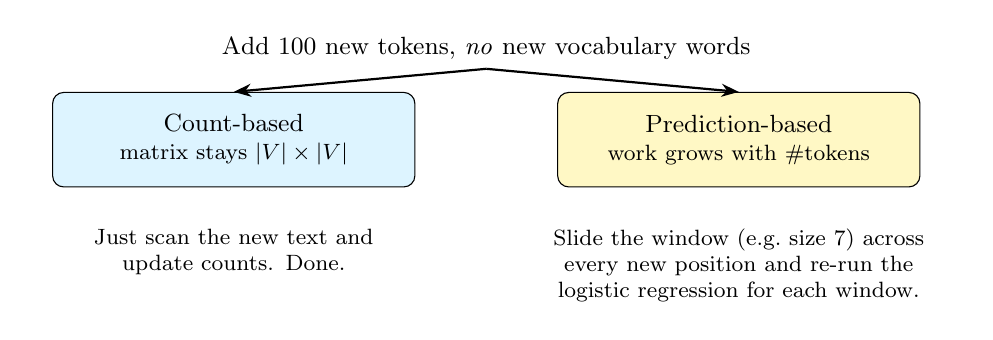
\begin{tikzpicture}[node distance=6mm]
  \node[box,fill=stageA,minimum width=46mm,minimum height=12mm] (c) {Count-based\\[-1pt]\footnotesize matrix stays $|V|\times|V|$};
  \node[box,fill=stageB,minimum width=46mm,minimum height=12mm,right=18mm of c] (p) {Prediction-based\\[-1pt]\footnotesize work grows with \#tokens};
  \node[above=9mm of $(c)!0.5!(p)$,font=\small] (top) {Add 100 new tokens, \emph{no} new vocabulary words};
  \draw[arr] (top.south) -- (c.north);
  \draw[arr] (top.south) -- (p.north);
  \node[below=4mm of c,font=\footnotesize,align=center,text width=50mm] {Just scan the new text and\\update counts. Done.};
  \node[below=4mm of p,font=\footnotesize,align=center,text width=55mm] {Slide the window (e.g.\ size 7) across\\every new position and re-run the\\logistic regression for each window.};
\end{tikzpicture}
\end{frame}

\begin{frame}{The best of both worlds}
\centering
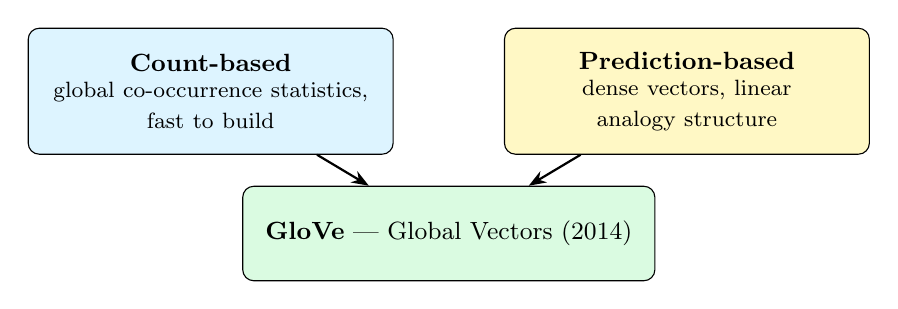
\begin{tikzpicture}
  \node[box,fill=stageA,text width=44mm,minimum height=16mm] (c) {\textbf{Count-based}\\\footnotesize global co-occurrence statistics,\\fast to build};
  \node[box,fill=stageB,text width=44mm,minimum height=16mm,right=14mm of c] (p) {\textbf{Prediction-based}\\\footnotesize dense vectors, linear\\analogy structure};
  \node[box,fill=stageD,text width=50mm,minimum height=12mm,below=12mm of $(c)!0.5!(p)$] (g) {\textbf{GloVe} --- Global Vectors (2014)};
  \draw[arr] (c) -- (g);
  \draw[arr] (p) -- (g);
\end{tikzpicture}
\vspace{4mm}

\small Proposed the year after word2vec by Christopher Manning's group at
Stanford: Jeffrey Pennington (postdoc) and Richard Socher (PhD student).
\end{frame}

% ---------------------------------------------------------------------
\section{Intuition: ratios of co-occurrence probabilities}

\begin{frame}{Step 1: build a co-occurrence matrix}
\begin{columns}[c]
\column{0.5\textwidth}
\begin{itemize}
  \item Same as the count-based approach: a \textbf{words $\times$ words}
        matrix $X$.
  \item Fix a window size; each time words $i$ and $j$ appear in the same
        window, increment $X_{ij}$.
  \item But we will \alert{not use the raw counts} directly.
\end{itemize}
\column{0.45\textwidth}
\centering
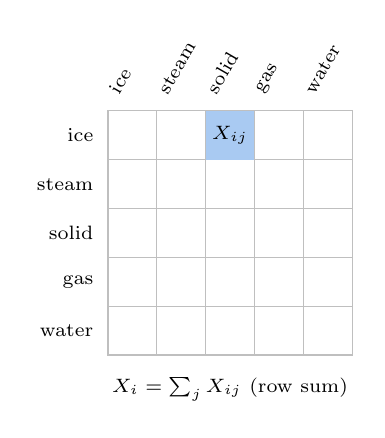
\begin{tikzpicture}[scale=0.62]
  \foreach \r in {0,...,4} \foreach \c in {0,...,4}
    \draw[gray!50] (\c,-\r) rectangle ++(1,-1);
  \foreach \w [count=\k from 0] in {ice,steam,solid,gas,water}{
    \node[font=\scriptsize,anchor=east] at (-0.1,-\k-0.5) {\w};
    \node[font=\scriptsize,rotate=60,anchor=south west] at (\k+0.3,0.05) {\w};
  }
  \fill[accent!35] (2,-0) rectangle ++(1,-1);
  \node[font=\scriptsize] at (2.5,-0.5) {$X_{ij}$};
  \node[font=\scriptsize,align=center] at (2.5,-5.7) {$X_i = \sum_j X_{ij}$ (row sum)};
\end{tikzpicture}
\end{columns}
\end{frame}

\begin{frame}{Step 2: probe two target words with context words}
\small
Target words from thermodynamics: \textbf{ice} and \textbf{steam}.
Every vocabulary word can act as a context (``pivot'') word; take four:

\vspace{3mm}
\centering
\begin{tabular}{@{}lcccc@{}}
\toprule
 & $k=$ solid & $k=$ gas & $k=$ water & $k=$ fashion \\
\midrule
$P(k \mid \textit{ice})$   & \hi & \lo & \hi & \lo \\
$P(k \mid \textit{steam})$ & \lo & \hi & \hi & \lo \\
\bottomrule
\end{tabular}

\vspace{4mm}
\raggedright
$P(j \mid i) = X_{ij} / X_i$ is read straight off the co-occurrence matrix
($i$ = target, $j$ = context).
\end{frame}

\begin{frame}{Step 3: take the ratio}
\centering
\begin{tabular}{@{}lcccc@{}}
\toprule
 & solid & gas & water & fashion \\
\midrule
$\dfrac{P(k \mid \textit{ice})}{P(k \mid \textit{steam})}$
  & $\dfrac{\text{high}}{\text{low}}$ & $\dfrac{\text{low}}{\text{high}}$
  & $\dfrac{\text{high}}{\text{high}}$ & $\dfrac{\text{low}}{\text{low}}$ \\[3mm]
  & \textcolor{okc}{\textbf{large}} & \textcolor{warn}{\textbf{small}}
  & $\approx 1$ & $\approx 1$ \\
\bottomrule
\end{tabular}

\vspace{4mm}
\raggedright
\begin{itemize}
  \item Ratio far from 1 $\Rightarrow$ the context word is \textbf{relevant}
        for telling ice from steam --- and its direction says which one
        (\emph{solid} $\to$ ice, \emph{gas} $\to$ steam).
  \item Ratio $\approx 1$ $\Rightarrow$ \textbf{not discriminative}: either
        related to both (\emph{water}) or to neither (\emph{fashion}).
\end{itemize}
\end{frame}

\begin{frame}{Why the ratio matters}
\begin{block}{The ratio tells us a lot}
\begin{itemize}
  \item Separates \textbf{important} context words from \textbf{less
        important} ones.
  \item Says \textbf{which target} each important context word belongs to.
  \item Raw probabilities alone can't do this: \emph{water} has a high
        probability with ice, yet it is useless for distinguishing ice
        from steam.
\end{itemize}
\end{block}
\vspace{2mm}
GloVe uses this philosophy to derive its training objective.
\end{frame}

% ---------------------------------------------------------------------
\section{Deriving the GloVe objective}

\begin{frame}{Model similarity with log co-occurrence probability}
For words $i, j$ we want to learn embeddings $\wv_i, \wv_j$ whose
\textbf{dot product} reflects the measured probability:
\[
  \wv_i^\top \wv_j \;=\; \log P(j \mid i) \;=\; \log \frac{X_{ij}}{X_i}
  \;=\; \log X_{ij} - \log X_i
\]
\vspace{-1mm}
{\small $X_{ij}$: number of times $i$ and $j$ co-occur; \quad $X_i$: count for word $i$ (sum of row $i$).}
\vspace{1mm}
\begin{alertblock}{Problem: asymmetry}
$P(j \mid i) \neq P(i \mid j)$, but $\wv_i^\top\wv_j = \wv_j^\top\wv_i$.
Swapping target and context gives a second equation:
$\;\wv_j^\top \wv_i = \log X_{ij} - \log X_j$
\end{alertblock}
\end{frame}

\begin{frame}{Symmetrise by adding the two equations}
\[
\begin{aligned}
  \wv_i^\top \wv_j &= \log X_{ij} - \log X_i \\
  \wv_j^\top \wv_i &= \log X_{ij} - \log X_j \\
  \cmidrule{1-2}
  2\,\wv_i^\top \wv_j &= 2\log X_{ij} - \log X_i - \log X_j
\end{aligned}
\]
\[
  \boxed{\;\wv_i^\top \wv_j \;=\; \log X_{ij}
     \;-\; \tfrac12 \log X_i \;-\; \tfrac12 \log X_j\;}
\]
\vspace{1mm}
The last two terms \textbf{do not depend on the co-occurrence} of $i$ and $j$ ---
each depends only on a single word.
\end{frame}

\begin{frame}{Absorb word-only terms into biases}
Treat each word-only term as a learned property of that word --- a
\textbf{bias}:
\[
  -\tfrac12 \log X_i \;\longrightarrow\; b_i \qquad\qquad
  -\tfrac12 \log X_j \;\longrightarrow\; b_j
\]
\[
  \wv_i^\top \wv_j + b_i + b_j \;\approx\; \log X_{ij}
\]
\begin{itemize}
  \item The biases are learned along with the vectors.
  \item They can also be dropped:
        $\wv_i^\top\wv_j \approx \log X_{ij}$.
\end{itemize}
\end{frame}

\begin{frame}{Turn it into a squared loss}
Goal: find vectors whose dot product (plus biases) mimics the count-based
quantity $\log X_{ij}$. Minimise the squared difference over all pairs:
\[
  J \;=\; \sum_{i,j} \Bigl( \wv_i^\top \wv_j + b_i + b_j - \log X_{ij} \Bigr)^2
\]
\begin{alertblock}{Still a problem}
Very large $X_{ij}$ (e.g.\ stop-word pairs) still get a
\textbf{disproportionate} say in the loss --- the same weakness as
count-based methods.
\end{alertblock}
\end{frame}

% ---------------------------------------------------------------------
\section{The weighting function}

\begin{frame}{Add a weight $f(X_{ij})$ to each term}
\[
  J \;=\; \sum_{i,j} \alert{f(X_{ij})}\,
      \Bigl( \wv_i^\top \cv_j + b_i + \tilde b_j - \log X_{ij} \Bigr)^2
\]
\begin{columns}[T]
\column{0.55\textwidth}
Choose any $f$ satisfying three properties:
\begin{enumerate}
  \item \textbf{Continuous}, and stays finite as $x \to 0$.
  \item \textbf{Non-decreasing}: never decreases as co-occurrence grows.
  \item \textbf{Relatively small for large $x$}: very frequent pairs must
        not get proportionally large weight.
\end{enumerate}
\column{0.42\textwidth}
\small
$f$ penalises pairs whose co-occurrence is too high --- e.g.\ stop-word
pairs --- relative to their raw count.
\end{columns}
\end{frame}

\begin{frame}{The GloVe weighting function}
\begin{columns}[c]
\column{0.5\textwidth}
\centering
\begin{tikzpicture}
\begin{axis}[
  width=70mm,height=50mm,
  axis lines=left,
  xlabel={$X_{ij}$}, ylabel={$f(X_{ij})$},
  xmin=0,xmax=150,ymin=0,ymax=1.25,
  xtick={100},xticklabels={$x_{\max}$},
  ytick={1},
  every axis label/.style={font=\small},
  tick label style={font=\small},
]
  \addplot[very thick,accent,domain=0:100,samples=80] {(x/100)^0.75};
  \addplot[very thick,accent,domain=100:150] {1};
  \addplot[dashed,muted] coordinates {(100,0) (100,1)};
\end{axis}
\end{tikzpicture}
\column{0.48\textwidth}
\begin{itemize}
  \item A \textbf{cutoff} $x_{\max}$.
  \item Below $x_{\max}$: rises almost linearly with the count.
  \item Above $x_{\max}$: weight is capped at \textbf{1} --- very frequent
        pairs get no extra weight.
  \item Any other $f$ meeting the three properties would also work.
\end{itemize}
\end{columns}
\end{frame}

\begin{frame}{The final GloVe objective}
\[
  \boxed{\;J \;=\; \sum_{i,j} f(X_{ij})\,
      \Bigl( \wv_i^\top \cv_j + b_i + \tilde b_j - \log X_{ij} \Bigr)^2\;}
\]
\begin{itemize}
  \item Minimise with gradient descent: take derivatives with respect to
        $\wv_i$ and $\cv_j$.
  \item As in word2vec, \textbf{two embeddings} are learned per word: one as
        target ($\wv$), one as context ($\cv$).
\end{itemize}
\vspace{2mm}
\begin{columns}[T]
\column{0.48\textwidth}
\begin{block}{From count-based}
$\log X_{ij}$ --- global co-occurrence statistics
\end{block}
\column{0.48\textwidth}
\begin{block}{From prediction-based}
$\wv_i^\top \cv_j$ --- dense vectors learned by gradient descent
\end{block}
\end{columns}
\end{frame}

\begin{frame}{GloVe in practice}
\begin{itemize}
  \item A \textbf{static} embedding: one vector per word type.
  \item Showed strong results across multiple tasks.
  \item \textbf{Fast to train} and \textbf{scalable} to huge corpora.
  \item Also performs well with a \textbf{small corpus} --- unlike word2vec.
\end{itemize}
\vspace{3mm}
\small Further reading: the original paper (Pennington, Socher \& Manning,
EMNLP 2014).
\end{frame}

% ---------------------------------------------------------------------
\section{What embeddings let you do}

\begin{frame}{Applications of GloVe}
\small\vspace{-2mm}
\begin{columns}[T]
\column{0.49\textwidth}
\begin{block}{Features for downstream models}
\begin{itemize}
  \item Sentiment, NER, POS tagging, text classification
  \item Initialise LSTM/CNN embedding layers (helps with little labelled data)
\end{itemize}
\end{block}
\begin{block}{Similarity \& retrieval}
\begin{itemize}
  \item Nearest neighbours: query expansion, synonyms
  \item Averaged vectors as cheap sentence vectors
\end{itemize}
\end{block}
\column{0.49\textwidth}
\begin{block}{Probing language}
\begin{itemize}
  \item Analogies and relation completion
  \item Measuring and reducing corpus bias
  \item Tracking meaning change over time
\end{itemize}
\end{block}
\vspace{-1mm}
\begin{alertblock}{Limitation}
One static vector per word: \emph{bank} (river) $=$ \emph{bank} (money).
Contextual models (BERT) fix this; GloVe stays a fast baseline.
\end{alertblock}
\end{columns}
\end{frame}

\begin{frame}{Linear analogies}
Beyond feeding downstream tasks, embeddings support interesting studies.
\vspace{3mm}
\begin{center}
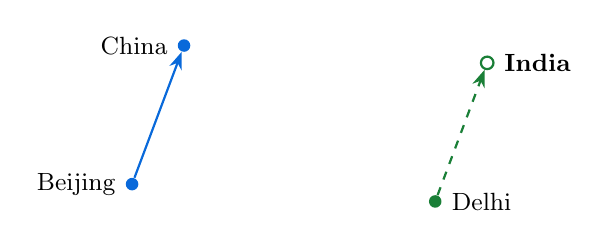
\begin{tikzpicture}[x=11mm,y=11mm,font=\small]
  \node[circle,fill=accent,inner sep=1.6pt,label=left:Beijing] (b) at (0,0) {};
  \node[circle,fill=accent,inner sep=1.6pt,label=left:China] (c) at (0.6,1.6) {};
  \node[circle,fill=okc,inner sep=1.6pt,label=right:Delhi] (d) at (3.5,-0.2) {};
  \node[circle,draw=okc,thick,inner sep=1.6pt,label=right:\textbf{India}] (i) at (4.1,1.4) {};
  \draw[arr,accent] (b) -- (c);
  \draw[arr,okc,dashed] (d) -- (i);
\end{tikzpicture}
\end{center}
\begin{itemize}
  \item \emph{Beijing} is to \emph{China} as \emph{Delhi} is to \underline{\quad}
        $\;\rightarrow\;$ \textbf{India}
  \item $\textit{king} - \textit{man} + \textit{woman} \approx \textit{queen}$
\end{itemize}
\end{frame}

\begin{frame}{Embeddings inherit bias}
The same analogy mechanism exposes biases learned from the corpus:
\vspace{3mm}
\begin{center}
\begin{tabular}{@{}lcl@{}}
\toprule
Query & & Returned \\
\midrule
\emph{father} : \emph{computer programmer} :: \emph{mother} : ? & $\rightarrow$ & \alert{homemaker} \\
\emph{man} : \emph{doctor} :: \emph{woman} : ? & $\rightarrow$ & \alert{nurse} \\
\bottomrule
\end{tabular}
\end{center}
\vspace{3mm}
Methods like word2vec and GloVe are \textbf{prone to bias} present in their
training text.
\end{frame}

\begin{frame}{Tracking meaning over time}
\begin{columns}[c]
\column{0.5\textwidth}
\begin{enumerate}
  \item Take e.g.\ New York Times articles, 1950--2010.
  \item Split by decade; train a separate GloVe (or word2vec) embedding on
        each.
  \item Pick a word and compare its \textbf{nearest neighbours} decade by
        decade.
\end{enumerate}
\column{0.46\textwidth}
\centering
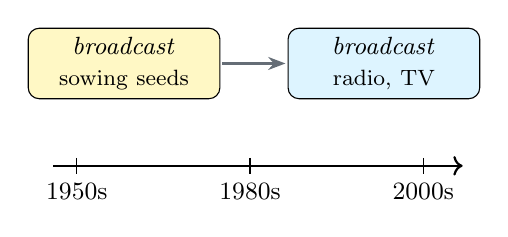
\begin{tikzpicture}[font=\small]
  \draw[thick,->] (0,0) -- (5.2,0);
  \foreach \x/\l in {0.3/1950s,2.5/1980s,4.7/2000s}{
    \draw (\x,0.1) -- (\x,-0.1);
    \node[below] at (\x,-0.1) {\l};
  }
  \node[box,fill=stageB,text width=22mm] at (0.9,1.3) {\emph{broadcast}\\\footnotesize sowing seeds};
  \node[box,fill=stageA,text width=22mm] at (4.2,1.3) {\emph{broadcast}\\\footnotesize radio, TV};
  \draw[arr,muted] (2.15,1.3) -- (2.95,1.3);
\end{tikzpicture}
\vspace{2mm}

\small The meaning of \emph{broadcast} drifted from agriculture to radio
and frequencies.
\end{columns}
\end{frame}

\begin{frame}{Summary}
\begin{itemize}
  \item Count-based: fast, statistically faithful, but sparse and dominated
        by frequent pairs. Prediction-based: dense and analogy-friendly, but
        cost grows with the corpus and ignores global counts.
  \item GloVe builds a co-occurrence matrix and learns vectors so that
        $\wv_i^\top\cv_j + b_i + \tilde b_j \approx \log X_{ij}$.
  \item Motivation: \textbf{ratios} of co-occurrence probabilities separate
        relevant from irrelevant context words.
  \item A weighting $f(X_{ij})$, capped at $x_{\max}$, stops frequent pairs
        from dominating.
  \item Embeddings enable analogies and diachronic studies --- and reflect
        corpus bias.
\end{itemize}
\vspace{2mm}
\textbf{Next:} word embeddings as inputs to neural language models and
Transformers.
\end{frame}

\end{document}
